% platex, uplatex 両対応.
\ifdefined\ucs
  %\documentclass[uplatex, report, a4j]{jsbook}
  %\documentclass[uplatex, 12pt, papersize]{jsbook}
  \documentclass[uplatex, 12pt, papersize, openany, dvipdfmx]{jsbook}
\else
  %\documentclass[report, a4j]{jsbook}
  %\documentclass[12pt, papersize]{jsbook}
  \documentclass[12pt, papersize, openany, dvipdfmx]{jsbook}
\fi


% =================================================== %
\def\emph#1{\textbf{\em{#1}}}
%-----------------------------------------------------------------%
\makeatletter% @付きのコマンドが使えるようにする。
%ファイル末尾で \makeatother で最後で解除すること
%-----------------------------------------------------------------%

% パッケージ読み込み部:開始
% 有用そうなのをいくつか列挙しておきます.
% 他にも様々あります.
%   参考URL:http://www.biwako.shiga-u.ac.jp/sensei/kumazawa/texindex.html

% 画像挿入用パッケージ: graphicx
% 文字等に色づけする場合に必要: color
% 
%   画像の利用方法 (png, jpg/jpeg, pdf、などが利用できる)
%   例 
%     \begin{figure}
%       \includegraphics[width=10cm,bb=0 0 600 600]{image/sample.png}
%     \end{figure}
%
%   注
%     []にて指定している値は,[表示横幅, bb=0 0 画像横pixel数 画像縦pixel数]です.
%     bb=以後は,ebbコマンドなどでsample.bbを作成しておけば不要です.
%     Windows : makebb.bat
%     @echo on
%      for %%i in (*.png)  do ebb %%i
%      for %%i in (*.pdf)  do ebb %%i
%      for %%i in (*.jpg)  do ebb %%i
%      for %%i in (*.jpeg) do ebb %%i
%
%     Linux / MacOSX : makebb.sh
%      #!/bin/sh -e
%      cd `dirname "$0"`
%      xbb *.pdf *.png *.jpg *.jpeg && ls *xbb | \
%      perl -ne 'chomp; ~s/\.xbb//g; print "mv $_.xbb $_.bb\n"' | \
%      sh 
%
% =======
%
\usepackage[dvipdfmx]{graphicx, color}

% 背景にすかし文字 (DRAFT) を表示 : pdfdraftcopy : graphicx に依存
%   提出用と間違えるのを予防
%   開発元URL: http://sarovar.org/projects/pdfdraftcopy/
%
% IsDraft が \def されている場合だけ有効
\@ifundefined{IsDraft}{}{\usepackage[watermark]{pdfdraftcopy}
\watermarkgraphic{images/draft_copy.pdf}}

% ブロックコメント
% \begin{comment} \end{comment}
\usepackage{comment}

% しおりの作成、目次や参考文献をクリッカブルリンクへ
% いろいろなパッケージと互換性問題があるようなので,他のパッケージを利用する場合にはチェックすること
% 依存関係情報: http://oku.edu.mie-u.ac.jp/~okumura/texwiki/?hyperref#z442922c
%
\usepackage[dvipdfm
	, bookmarks=true
	, bookmarksopen=true
 	, bookmarksnumbered=true
	, CJKbookmarks=true
%
	, backref=true
	, pdfborder={0 0 0} % width
%
	, colorlinks=false
	, frenchlinks=false
%	, linkbordercolor={1 1 1} % RGB
%	, citebordercolor={1 1 1} %RGB
%	, urlbordercolor={1 1 1} %RGB
%	, pdfhighlight=/I
]{hyperref}
% しおりの文字化け解消.必要な文字コード指定を入れる.
%\AtBeginDvi{\special{pdf:tounicode 90ms-RKSJ-UCS2}}% SJIS 
%\AtBeginDvi{\special{pdf:tounicode EUC-UCS2}} % EUC
%\AtBeginDvi{\special{pdf:tounicode UTF8-UCS2}} % UTF-8
%
% 文字コードを自動判定してしおりの文字化けを解消できるパッケージ.
% 上のオプションをオフにしてこちらを使ってもよい.
\usepackage{pxjahyper}
%
% PDFのメタ情報を設定したければ以下を追加
%\hypersetup{
%	pdftitle={タイトル},
%	pdfsubject={小見出し},
%	pdfauthor={PDF制作者名},
%	pdfkeywords={キーワード1; キーワード2; キーワード3;},
%}

% urlをそのまま表記可能にする.
%   本来であれば><%#^~などはエスケープしないといけない
%   また、1 word として認識されるために、自動で折り返してくれないURLを、
%   途中で折り返しをしてくれる。
%
% 使い方:
%    \url{http://www.ubi.cs.ritsumei.ac.jp}
%    \url{<a href=``http://www.ubi.cs.ritsumei.ac.jp''>Link</a>}
\usepackage{url}
\urlstyle{rm}
% 数式パッケージ
%   美文書作成などを参照してください.
%\usepackage{amsmath, amssymb}

% 表用パッケージ
%   きれいな表が書けます.
%   参考URL: http://www.biwako.shiga-u.ac.jp/sensei/kumazawa/tex/hhline.html
\usepackage{hhline, multirow}

% 表の見栄えを良くする
% 表の架線が上下だけ太くなります.
%   参考URL: http://www.biwako.shiga-u.ac.jp/sensei/kumazawa/tex/booktabs.html
\usepackage{booktabs}

% いろいろな囲み線作成用
%   様々な場面で利用できます.便利です.
%   参考URL: http://www.biwako.shiga-u.ac.jp/sensei/kumazawa/tex/fancybox.html 
%   参考URL: http://www.biwako.shiga-u.ac.jp/sensei/kumazawa/tex/ascmac.html
\usepackage{fancybox, ascmac}

% 可換図を書けるように
%   参考URL: http://www.biwako.shiga-u.ac.jp/sensei/kumazawa/tex/amscd.html
% \usepackage{amscd}

%% 以下、私作のコマンド
\usepackage{here}
\usepackage{bm}

%
% \TS{hoehoge}: パラグラフのトピックセンテンスを指定
% \listofts: トピックセンテンスを抽出してリスト化: 目次のような感じ
%
% \TODO{}: TODO を出力 (赤色で TODO: hogehoge)
% \listoftodo: TODOを抽出してリスト化: 目次のような感じ
%
%%%%%%%%%%%%%%%%%%%%%%%%%%%%%%%%%%%%%%%%%%%%%
%
\def\RED#1{{\color{red}#1}}%
%
\def\TS#1{\AddToContLine{lots}{#1}#1}%
\newcommand{\listtsname}{Paragraph Topic Sentenses (\RED{for Debug})}%
\newcommand{\listofts}{\listof{ts}}%
%
\newcommand{\TODO}{\secdef\@TODO\@sTODO}%
\def\@TODO[#1]#2{\@sTODO{#2}\@ifundefined{PrintTodo}{}{\\}}%
\def\@sTODO#1{\AddToContLine{lotodo}{#1}\@ifundefined{PrintTodo}{}{\RED{TODO: #1}}}% started TODO means [ \TODO*{hogehoge} ]
\newcommand{\listtodoname}{List of TODO (\RED{for Debug})}%
\newcommand{\listoftodo}{\@ifundefined{PrintTodo}{}{\listof{todo}}}%
\newcommand{\forceListoftodo}{\listof{todo}}%
%
%
%%%%%%%%%%%%%%%%%%%%%%%%%
\def\listof#1{%
  \if@twocolumn\@restonecoltrue\onecolumn%
  \else\@restonecolfalse\fi%
  \abstract{{\csname list#1name\endcsname}}%
  \@mkboth{{\csname list#1name\endcsname}}{}%
  \@starttoc{lo#1}%
  \if@restonecol\twocolumn\fi%
}%
\def\AddToContLine#1#2{%
\@ifundefined{c@atcl#1}{\newcounter{atcl#1}[chapter]}{}%
\ifnum \csname c@atcl#1\endcsname =0 % chapter用のダミーを追加
  \refstepcounter{atcl#1}%
  \addcontentsline{#1}{chapter}{\protect\numberline{\@chapapp\thechapter\@chappos}}%
\fi%
\ifnum \c@section>0 %
  \ifnum \c@subsection >0 %
    \ifnum \c@paragraph >0 %
      \ifnum \c@subparagraph >0 %
        \AddToContLineSec{#1}{subparagraph}{#2}%
      \else\AddToContLineSec{#1}{paragraph}{#2}\fi%
    \else\AddToContLineSec{#1}{subsection}{#2}\fi%
  \else\AddToContLineSec{#1}{section}{#2}\fi%
\else%
  \ifnum \csname c@atcl#1\endcsname >0 %
    \addcontentsline{#1}{section}{\protect\numberline{}#2}%
  \else%
    \refstepcounter{atcl#1}%
    \addcontentsline{#1}{chapter}{\protect\numberline{\@chapapp\thechapter\@chappos}#2}%
  \fi%
\fi%
}%
\def\AddToContLineSec#1#2#3{%
  \@ifundefined{c@atcl#2#1}{\newcounter{atcl#2#1}[#2]}{}
  \ifnum \csname c@atcl#2#1\endcsname >0 %  各セクションの一番始めで無ければ章番号無し
    \addcontentsline{#1}{#2}{\protect\numberline{}#3}%
  \else%
    \refstepcounter{atcl#2#1}%  セクションの一番始めであれば章番号付き
    \addcontentsline{#1}{#2}{\protect\numberline{\csname the#2\endcsname}#3}%
  \fi%
}%
%
\def\BoldFirstRef#1#2{\@ifundefined{c@#1}{\newcounter{#1}\textbf{#2}}{#2}}%
\@ifundefined{figref}{\def\figref#1{\BoldFirstRef{figref#1}{図 \ref{#1}}}}{}% 図出力
\@ifundefined{tabref}{\def\tabref#1{\BoldFirstRef{tabref#1}{表 \ref{#1}}}}{}% 表出力
\@ifundefined{secref}{\def\secref#1{\ref{#1} 節}}{}%
\@ifundefined{chapref}{\def\chapref#1{第 \ref{#1} 章}}{}%
\def\SetJsDescriptionIndent#1{%
%%%%%%%%%%%%%%%%%%%%%%%%%%%%%
\renewenvironment{description}{%
  \list{}{%
    \leftmargin=#1
    \labelwidth=\leftmargin
    \labelsep=1zw
    \advance \labelwidth by -\labelsep
    \let \makelabel=\descriptionlabel}}{\endlist}
%%%%%%%%%%%%%%%%%%%%%%%%%%%%%
}%
\def\abstract#1{%
\chapter*{#1}\@mkboth{#1}{}%
\@ifundefined{c@abstract}{\newcounter{abstract}\pagenumbering{roman}}{}%
}%
\def\startMain{%
\if@openright\cleardoublepage\else\clearpage\fi%
\pagenumbering{arabic}%
}
%-----------------------------------------------------------------%
%-----------------------------------------------------------------%
%
%
\def\BachelorThesis{卒 業 論 文}
\def\MasterThesis{修 士 論 文}
\def\DoctoralThesis{博 士 論 文}
\def\@thesisTitle{圧力センサ搭載ヘルメットを用いた\\本人認証手法の提案}
\def\@thesisSupervisor{卒業研究3 (1O):双見 京介,村尾 和哉 担当} % 卒業研究3のクラス名と担当教員名を記載
%\def\@thesisSupervisor{卒業研究3 (1H):西尾 信彦 担当}
\def\@thesisKind{\MasterThesis}
\def\@thesisYear{2019年}
%\def\@thesisYear{2019年}
%\def\@thesisEraName{平成XX年}
\def\@thesisSemester{秋学期} % 秋か春を記載
%\def\@thesisSemester{秋学期}
\def\@thesisAuther{藤井 敦寛}
\def\@thesisNameOfGraduateSchool{立命館大学大学院}
\def\@thesisNameOfUnderGraduate{立命館大学 情報理工学部}
\def\@thesisNameOfMajor{情報理工学研究科情報理工学専攻}
\def\@thesisNameOfGrade{情報システム学科 4回生 2600160357-3} % 2017年度入学者はコース名に変更
%\def\@thesisNameOfGrade{情報システム学科 4回生 2600xxxxxxxx}
\def\thesisTitle#1{\gdef\@thesisTitle{#1}}
\def\thesisKind#1{\gdef\@thesisKind{#1}}
\def\thesisYear#1{\gdef\@thesisYear{#1}}
\def\thesisEraName#1{\gdef\@thesisEraName{#1}}
\def\thesisAuther#1{\gdef\@thesisAuther{#1}}
\def\thesisNameOfGraduateSchool#1{\gdef\@thesisNameOfGraduateSchool{#1}}
\def\thesisNameOfMajor#1{\gdef\@thesisNameOfMajor{#1}}
\def\makeThesisTitle{
\begin{titlepage}%
\centering
\begin{minipage}[]{\fullwidth}
\large
 

% 表紙の配置や文字のサイズは以下で調整
\vspace{6mm}
{\@thesisYear}度({\@thesisSemester})\\
{\@thesisSupervisor}\\%
\begin{center}
\vspace{2mm}
{\Large {\@thesisKind}}\\
\vspace{27mm}
%
{\LARGE {\@thesisTitle}}\\%
\vspace{84mm}%
{\@thesisNameOfUnderGraduate}\\%
%{\@thesisNameOfGraduateSchool}\\%
{\@thesisNameOfGrade}\\%
%{\@thesisNameOfMajor}\\%
%
\vspace{7mm}%
{\Large {\@thesisAuther}}%
\end{center}%
\end{minipage}%
\end{titlepage}%
}
%
%-----------------------------------------------------------------%
\makeatother%
%-----------------------------------------------------------------%
 % 普段使っているパッケージいろいろ

%% 追加
\usepackage{pdfpages}
\usepackage{bm}
\usepackage{url}
\usepackage{color}
\usepackage{multirow}
\usepackage{amsmath}
\usepackage[T1]{fontenc}
\usepackage[subrefformat=parens]{subcaption}
\captionsetup{compatibility=false}
\renewcommand{\today}{\the\year/\the\month/\the\day}
\renewcommand{\contentsname}{CONTENTS}
\renewcommand{\listfigurename}{LIST OF FIGURES}
\renewcommand{\listtablename}{LIST OF TABLES}
\renewcommand{\figurename}{Fig. }
\renewcommand{\tablename}{Table. }
\renewcommand{\prechaptername}{CHAPTER }
\renewcommand{\postchaptername}{}
\renewcommand{\bibname}{REFERENCES}
%% ここまで
% =================================================== %
%
% subsection まで目次に出力
\setcounter{tocdepth}{2}

\begin{document}
\pagenumbering{roman}

\thesisKind{\MasterThesis} % \BachelorThesis or \MasterThesis or \DoctoralThesis

% \makeThesisTitle

\includepdf[pages=-]{title.pdf}

\abstract{Abstract}
  The extensive research on wearable devices has led to devices with various shapes and mounting locations. Wearable devices are often used to record the user's biometric information, and methods have been proposed to detect physical abnormalities from the acquired data. Among various kinds of biometric data, pulse data has been used in methods such as heart rate monitoring and emotion recognition. The most common type of pulse sensor uses photoplethysmography (PPG), which irradiates a green LED on the skin and measures pulse data from changes in the light reflected from blood vessels. PPG sensors have been implemented in commercially available wearable devices such as smartwatches. However, a PPG sensor requires blood flow for data acquisition, and when a smartwatch is worn on an artificial body part such as a prosthetic hand or a robotic arm, data cannot be acquired because there is no blood flow. In this study, I propose a method that enables a PPG sensor to measure arbitrary pulse data by using a display. If this method is successful, it will enable pulse data measured at the junction of a living limb and an artificial limb to be input to the display; then, a smartwatch attached to the artificial limb will read the same pulse data. In this thesis, I focus on the heart rate and report the results of an experiment in which a target heart rate was input and the display was controlled accordingly to determine whether the target heart rate could be obtained by a smartwatch. I implemented a display drawing program and conducted the evaluation with five kinds of smartwatches and four kinds of displays. The results showed that the error between the target heart rate and the heart rate acquired by the smartwatch was within $3$ beats per minute (bpm) in many cases when the target heart rate was set to 60--100 bpm. When the target heart rate was set to 40--55 and 105--200 bpm, the heart rate could also be input to the smartwatch with a small error under certain conditions. Moreover, when generated PPG data was imported into heart rate variability (HRV) analysis software, it was recognized as a pulse wave in the same way as real PPG data obtained from a person. I compared the heart rate, RR interval, and SDNN calculated from the real and generated PPG data, and I confirmed that the proposed method could generate stable PPG data. On the other hand, when the waveforms were compared, the generated PPG waveform differed greatly from the real PPG waveform, which indicated that the software could calculate the heart rate, RR interval, SDNN, and LF/HF ratio regardless of the waveform. This result suggests that calculation of these parameters without verifying the waveform would be vulnerable to an attack with fake PPG data.

\tableofcontents % 目次
\listoffigures % 図目次
\listoftables % 表目次

%本文開始
\startMain

\chapter{はじめに}
\label{introduction}
現在販売されている四輪車の多くにスマートキーシステムが導入されている.スマートキーシステムとは,キーをポケットなどに入れて接近するとキーから発せられる電波を車が感知してドアの解錠を行い,離れるとドアの施錠を行う機能である.キーを持ったままボタンを押すだけでエンジンを始動することもできる.スマートキーシステムは二輪車にも導入されつつある.二輪車におけるスマートキーシステムも四輪車と同様に,キーを所持しておくだけでキーシリンダーにキーを挿し込む手間なく,ラゲッジスペースと呼ばれる荷物を収納するスペースの解錠やエンジンの始動を可能にする機能である.しかしながら,スマートキーシステムはキーを所持しておかなければならず,キーの紛失や第三者がキーを入手することで車両盗難のリスクがある.\par

物理的な鍵以外で本人を認証する手法として,パスワードなどの知識や筆跡などの行動的特徴,指紋などの身体的特徴を用いる手法がある.当麻ら\cite{face}はステレオカメラを用いた顔認証システムを提案しており,ヘルメット装着前に二輪車に取り付けられたカメラの方を向くことで実現可能であると考えられる.しかし,カメラの電源を入れてカメラの方を向く必要があり,二輪車を運転するたびにこのような操作を行うのは面倒である.また,本人の写真やお面で認証を破ることができるリスクもある.このほか,指紋認証のアプローチもあるが,指紋は写真などから簡単に複製されるリスク\cite{finger_print}がある.\par

本研究では,二輪車での走行において法令で装着が義務付けられているヘルメットに着目し,ヘルメットを用いた本人認証が実現できれば,既存のキーを用いたシステムの問題点を解決できると考え,搭乗者が圧力センサを搭載したヘルメットを装着することで,搭乗者の頭部形状にもとづき本人認証をする手法を提案する.頭部形状は個人ごとに異なり,頭部形状の取得や複製は困難であると考える.具体的には,あらかじめ車両とペアリングして所有者の頭部形状データを登録しておいたヘルメットを二輪車のヘルメットロックに装備しておく.ヘルメットロックに繋がったまま利用者がヘルメットを装着し,取得した頭部形状と事前に登録した頭部形状が一致すればロックが外れ,エンジンを始動できるようになるという想定である.\par

提案手法によって利用者は何も持たずに乗車できるため,キーの紛失や盗難のリスクを減少させることができる.一方で,登録された利用者以外がヘルメットをかぶった場合は本人として認証されず,ヘルメットロックも外れず,エンジンの始動もできないため,車両盗難のリスクも減少させることができる.\par

以降本稿では,\ref{related}章で関連研究を紹介する.\ref{method}章で提案手法を説明し,\ref{make}章で実装について述べる.\ref{evaluation}章で提案手法の評価実験と結果の考察を行い,最後に\ref{conclude}章で本研究をまとめる.
\chapter{関連研究}
\label{related}
本章では個人認証手法,頭部装着型デバイス,頭部状態認識に関する研究を紹介する.
\section{個人認証手法}
%車両にカメラを取り付ける手法
当麻ら\cite{face}はステレオカメラを用いた顔認証システムを提案している.既存の顔認証システムではカメラに意識して顔を向ける必要があった.その問題を解決するため,少数の正面を向いていない顔画像から正面顔画像を作成し,個人認証を行う手法を提案している.佐藤ら\cite{door}は掌紋認証を装備したインテリジェントドアノブシステムの開発をしている.このシステムでは,認証に特別な動作を必要とする煩わしさを解決するため,ドアノブにカメラを装着し掌紋の画像を取得する.得られた画像からSIFT特徴を用いて認証を行う.

%ヘルメットでのジェスチャー認証
成ケ澤ら\cite{acceleration}はスマートフォン内蔵の加速度センサとジャイロセンサを用い,ユーザがスマートフォンを手のひらの上で回転させる動作を行うことで,その加速度と角速度の特徴量から認証する手法を提案している.

%ヘルメットに搭載可能な別認証手法
白川ら\cite{iris_eye}は虹彩と目の周辺画像を統合して認証する手法を提案している.虹彩認証は高画質の画像を必要とし,至近距離で認証を行う必要があり,被認証者に負担を与えてしまう.そこで目頭や目尻,まぶたの形などに個人差が存在することに注目し,目の周辺の分割画像を利用して目の周辺認証を行い,虹彩と統合する認証を提案した.岸里ら\cite{mouth_pattern}は口唇領域の動きの画像認識を用いたスマートデバイス向けパターンロックシステムを提案している.スマートフォンやタブレット端末のパターンロック認証は,肩越しに画面を覗き見るショルダーハックや,画面に残った脂の跡を読み取ることによって,認証キーを盗まれてしまうリスクをもつ.そこで手の指の代わりに,端末のカメラで口唇領域の動きを認識し,画面に触れることなく認証を行うシステムを提案した.越前ら\cite{finger_print}は写真からの指紋復元の脅威とその対策技術を提案している.指紋認証には複製の恐れがあり,少ない写真でも簡易に複製が可能である.そのため,指にジャミングパターンを装着する対策技術を提案した.

%上記の認証手法へのダメ出しと提案手法の強み
これらは個人認証の手法であり,いずれも二輪車のキーとして応用ができる可能性がある.顔認証を行う場合,カメラをあらかじめ車両に取り付けておき,ヘルメットを装着する前にカメラの方を向くことでシステムを実装することが可能である.掌紋画像での認証の場合は二輪車のハンドルにカメラを取り付けることで実装可能である.しかし,どちらの手法も悪天候による水没,走行時の衝撃からの耐久性を考慮しなければならない.また,認証時にカメラの電源を入れる手間が生じる.したがって,カメラを車両に取り付ける必要のある手法は向かない.ジェスチャ認証の場合,ヘルメットに加速度センサとジャイロセンサを搭載することで,ヘルメットを被るまでの動作の加速度と角速度の特徴量を用いて認証できる可能性がある.しかしながら,急いでいて動作が速くなる場合や,雨天時にヘルメットの内装が濡れないように気をつけながら装着する場合など,ヘルメットを装着する動作が変化する可能性が考えられる.状況の変化を考慮すると,ヘルメットを静止させたまま認証が可能な手法が適切である.

目を用いた認証手法の場合,ヘルメットを動かすことなく認証が可能である.しかし,虹彩や目の周辺の分割画像を取得するには目の前付近にカメラを設置する必要がある.そのため,ヘルメットに実装する場合,視界を遮る恐れがある.口唇領域の画像であれば視界を遮らずに撮影できるが,ヘルメットの口元の空間は限られる.そのため,口とカメラの距離が近くなってしまい,1個のカメラで口唇領域の動きを判別することは難しくなる.カメラの数を増やすとヘルメットの重量増加に繋がる.

そこで,本研究では内装に圧力センサを搭載したヘルメットを装着することで,頭部形状を取得して個人認証する手法を提案する.提案手法は個人認証のために特別な動作を必要とせず,デバイスの搭載によって視界を遮ることもない.さらに,認証に用いる頭部形状を複製するには立体形状を正確に把握する必要があり,複製が困難である.

\section{頭部装着型デバイス}
%デバイスとしての新規性
田中ら\cite{glasses}はメガネ型デバイスを用いた経皮水分蒸散量の常時測定システムを提案している.皮膚状態の診断には経皮水分蒸散量などの定量的な指標が用いられるが,測定には高価な機器が必要で,また定常的な測定はできない.そこで,定常的に測定を行い皮膚の健康維持を支援するため,メガネ型デバイスに2つの温度・湿度センサを装着し,皮膚状態の評価指標である経皮水分蒸散量の常時測定を行うシステムを提案した.石井ら\cite{happymouth}は人間の対面コミュニケーション能力を拡張するマスク型デバイス「HappyMouth」を提案している.このシステムでは,マスクに小型ディスプレイが内蔵されており,口元の映像を提示できる.映像提示の機能として,ユーザが自分の好みの口を選択して表示する機能,ユーザの発話をテキスト化して字幕表示する機能,ユーザの発したキーワードをインターネットで画像検索した結果を表示する機能がある.新島ら\cite{cap_sensor}は左右の側頭筋の筋活動を測定することができる,導電性高分子の布電極を用いた帽子型筋電センサhitoeCapを提案している.これは食事や睡眠や運動などの日々の生活の様々な場面で活動する,咀嚼筋の一つである側頭筋の筋電データを測定すれば,ユーザのライフログとして活用できると考え提案された.これらの研究はいずれも頭部に装着するデバイスであり,様々な形状のデバイスが提案されている.しかしながら,頭部装着型デバイスとしてヘルメットを用いた研究は筆者の知る限り存在しない.

\section{頭部状態の認識}
%頭部形状を認識するという点での新規性
近年注目されているヒアラブルデバイスにおいて求められる機能のひとつとして,手や視界を占有することのないデバイス操作機能が挙げられる.既存の製品や既存の研究では認識精度や認識できるジェスチャの種類,頑健性などの点で課題が残る.これらの課題を解決するために雨坂ら\cite{ear}は首,顎,顔の状態(頭部状態)にともなって外耳道が変形することに着目し,外耳道インパルス応答を測定することで頭部状態を認識する手法を提案した.一方,状況の変化に関して口周辺の動作に着目すると,感情や咀嚼といった様々な情報が含まれており,これらを認識することで感情の記録や,咀嚼カウントによる肥満防止など,新たなコンテキストアウェアサービスが提供できる.そこで,山下ら\cite{mouth}は日常生活での利用を想定し,安価な付け髭型デバイスを用いた口周辺の形状変化によるコンテキスト認識手法を提案した.これらの研究は表情や動作などの動的な情報を取得するものであり,対して本研究は静的な頭部形状そのものの特徴を取得するという点で異なる.
\chapter{Proposed Method}
\label{sec:method}

% 3.1
\section{Overview}
In my proposed method, when a user sets an arbitrary heart rate, a display lights up, and a smartwatch worn over the display measures the specified heart rate. Figure \ref{fig:method} illustrates the process flow of the proposed method. First, the user's real (target) heart rate is obtained by a PPG sensor that is separate from the smartwatch. Next, the brightness of the display, which is connected to a microcomputer, is changed according to the target heart rate. Finally, the smartwatch measures the heart rate indicated by the display, which is the same as the target heart rate.

\begin{figure}[!t]
  \centering
  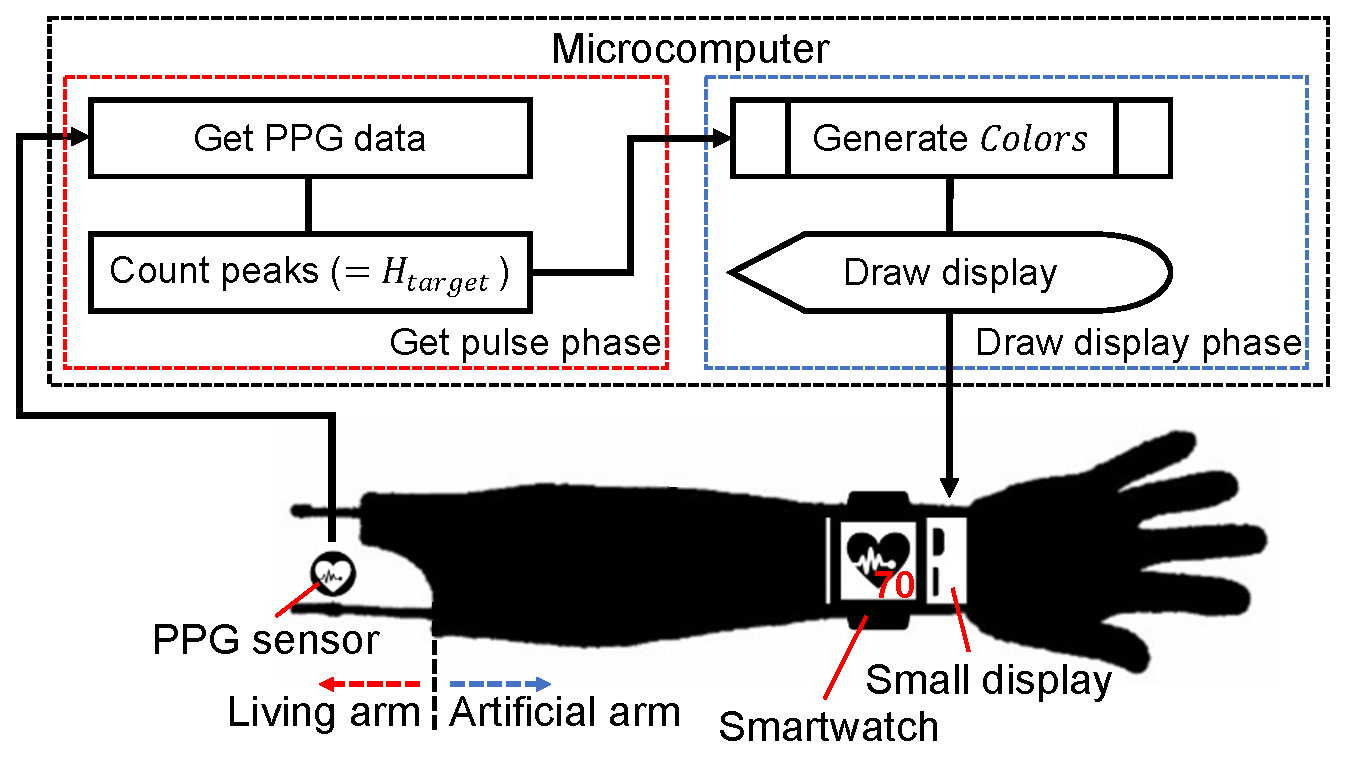
\includegraphics[width=1\linewidth]{figures/method.eps}
  \caption{Process flow of the proposed method.}
  \label{fig:method}
\end{figure}


% 3.2
\section{Target Heart Rate Calculation}
I denote the target heart, which is determined from the wearer's heart rate, as $H_{target}$. It is computed from two thresholds, $Threshold_{value}$ and $Threshold_{time}$, by using the PPG sensor, which constantly measures data. By using this data, the system records the times of pulse peak occurrences. A peak is detected when the PPG data measured in real time exceeds $Threshold_{value}$, but not until more than $Threshold_{time}$ time has passed since the last peak occurred. In this work, $Threshold_{value}$ and $Threshold_{time}$ were heuristically set to 700 and 0.3, respectively; in practice, however, they should be adjusted according to the environment in which the system is used. When a peak is detected, the time difference from the previous peak occurrence time is calculated. Here, the time difference refers to the RR interval, denoted as $RR$ [s], which is the time between one ventricular activation and the next. The number of times the ventricles contract in one minute is the heart rate in beats per minute (bpm). Therefore, if the RR interval is known, the heart rate $H_{target}$ can be calculated by the following equation:
\begin{equation}
  \label{eqn:target}
  H_{target} = int(60 / RR).
\end{equation}
The system continuously updates this value.\par

$H_{target}$ can also be set manually if the user wants the smartwatch to measure a specific heart rate. Figure \ref{fig:system} shows a system implementation in which the target heart rate is manually set from a control application and the heart rate is input to the smartwatch on an artificial arm.

\begin{figure}[!t]
  \centering
  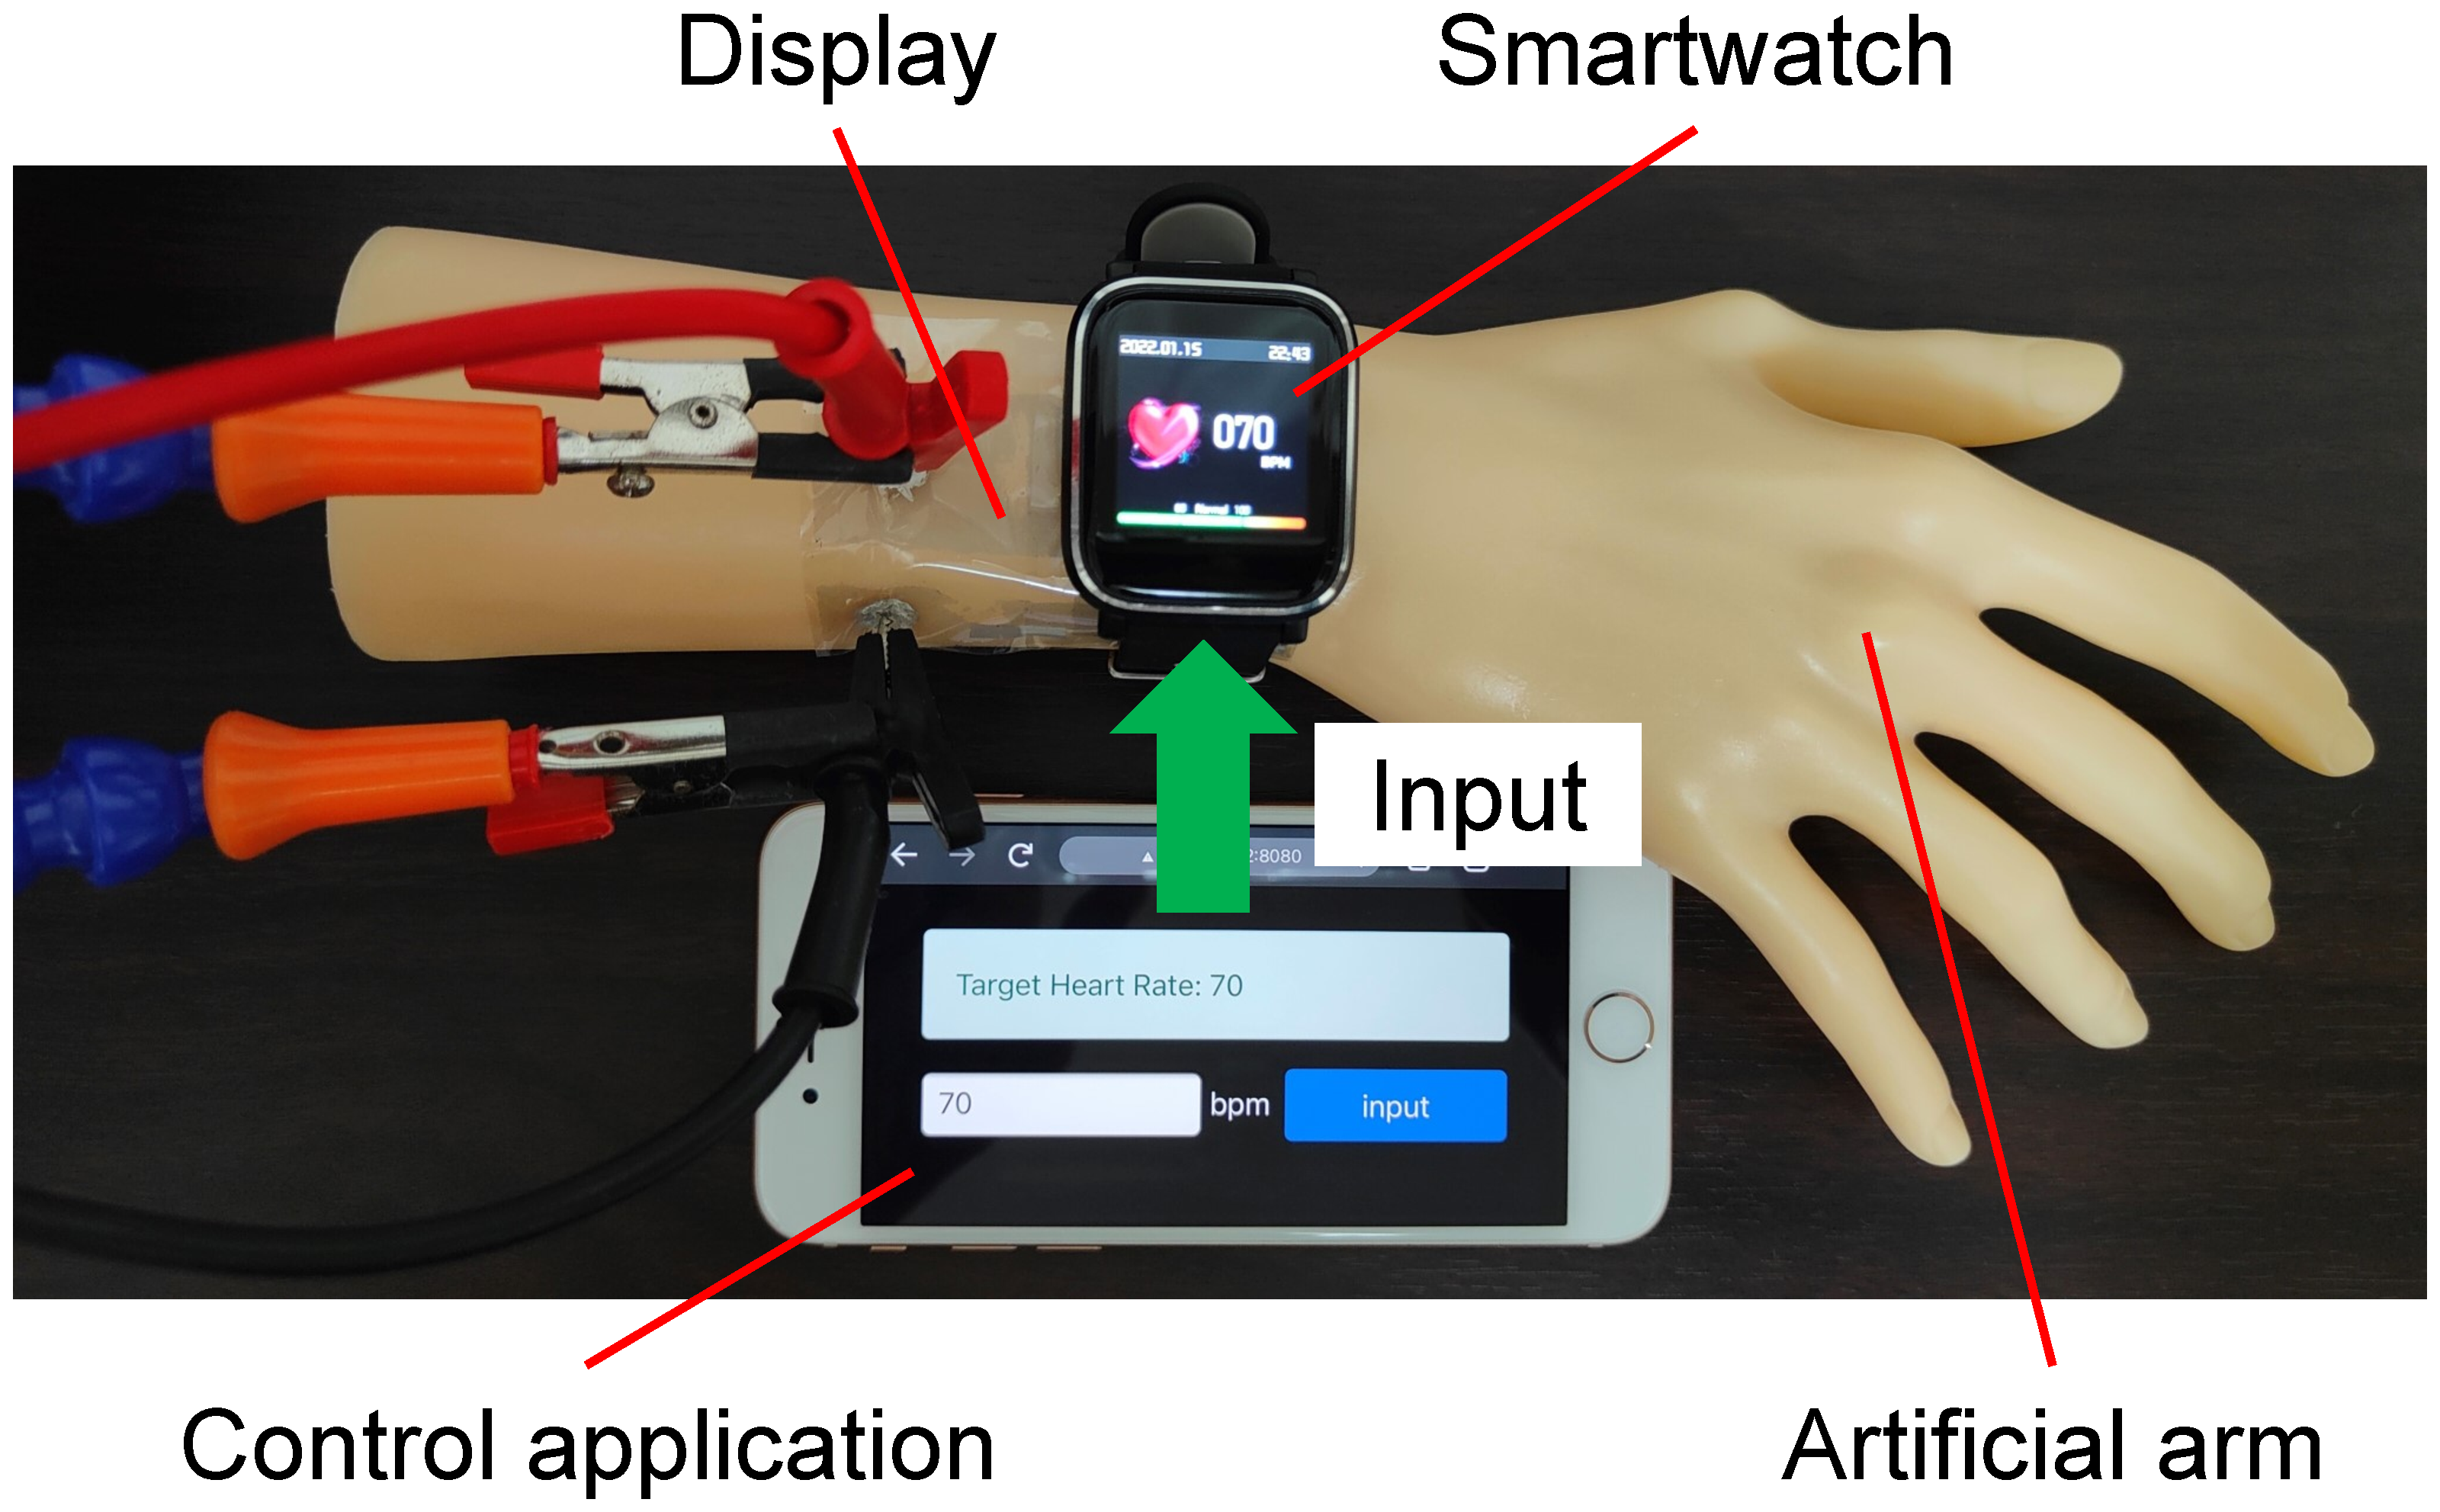
\includegraphics[width=1\linewidth]{figures/system.eps}
  \caption{System implementation in which the target heart rate is manually set from a control application and the heart rate is input to the smartwatch on an artificial arm.}
  \label{fig:system}
\end{figure}


% 3.3
\section{Display Control}
Next, the display's brightness is controlled so that the heart rate measured by the smartwatch matches $H_{target}$. An array, denoted as $Colors$, is prepared in advance to store the required brightness for the smartwatch to detect a single pulse peak.\par

PPG sensors use LEDs to irradiate infrared, red, or green light onto the skin and measure pulse data from changes in the light reflected from the blood vessels. Because blood flow increases with the timing of the pulse, the blood vessels absorb more light, and the reflected light becomes dimmer. Because black absorbs more light than white, as the display is rendered blacker, the light emitted from the smartwatch and reflected by the display becomes darker.\par

Hence, the proposed method draws the values in $Colors$ on the display one by one during each drawing interval $T$ [s]. I set $T$ for each value in $Colors$ as follows, so that $Colors$ is applied $H_{target}$ times in one minute:
\begin{equation}
  \label{eqn:wait}
  T = 60 / \{len(Colors) * H_{target}\},
\end{equation}
where $len(Colors)$ is the data length of $Colors$.


% 3.4
\section{Pulse Data Measurement}
Finally, in the proposed method, pulse data is measured by the smartwatch worn over the blinking display. Such pulse data measured by a PPG sensor on a smartwatch can be used in various applications. However, the performance of the PPG sensor and the algorithm for measuring pulse data vary among different smartwatch models and are not publicly accessible. Accordingly, I manually set the target heart rate in my evaluation experiment described below.

\chapter{評価}
\label{evaluation}
本章では,提案手法の有効性を評価するために行った実験について説明する.

\section{データ収集}
被験者9名(A$\sim$I,全員男性,平均年齢23歳)に実装したヘルメットを装着させ,サンプリングレート約30Hzでセンサデータを収集した.2秒間装着して取り外し再び2秒装着する試行を1セットとして被験者1人あたり10セット,合計20回装着するデータ(2秒$\times$2回$\times$10セット)を収集した.データの収集は1人当たり1日最大4セットとし,複数日に渡ってデータを収集した.センサと頭部のさまざまな位置関係のデータを収集するために,セット間に30分以上の休憩時間を設けた.1回2秒間32次元の装着データの時間平均値を算出し,1回の装着から32次元のベクトルを1サンプル得る.つまり,被験者1人あたり20サンプルを取得した.

\section{結果と考察}
収集したデータに対して,1名を本人,8名を他人として,収集した本人のデータの80\%を登録し,20\%のデータを用いて本人の認証精度を計測した.また,8人すべてのデータを用いて他人の認証精度を計測した.登録データは5分割交差検証を行い評価した.

識別結果の評価指標として,FRR,FAR,EERを用いる.FRR(False Reject Rate:本人棄却率)は誤って本人を他人であると判断し拒否してしまう割合であり,FAR(False Accept Rate:他人受入率)は誤って他人を本人であると判断し認証してしまう割合である.閾値を小さくするほどFRRが増加し,閾値を大きくするほどFARが増加する.FRRとFARはトレードオフの関係にあり,FRRとFARが同値になるときの値をEER(Equal Error Rate:等誤り率)と呼ぶ.通常,EERの値で本人認証の性能を評価し,EERが小さいほど精度が良い.被験者ごとに閾値を変化させてEERを計測した.

各被験者および9人の平均EERを表\ref{EER_num}に,FRRとFARを図\ref{EER}に示す.Totalは被験者全員の平均を示している.
表\ref{EER_num}より被験者A,E,G,IのEERはおおよそ0.01以下と良い結果が得られた.これは,検証に用いたデータセットにおいて,本人は100回に1回以下の割合で認証に失敗し,他人は100回に1回以下の割合で認証を突破することを意味している.文献\cite{face_auth}において,顔認証のEERが0.012であると報告されていることを考慮すると,これらの被験者については同等の性能が得られたといえる.被験者Eについては,他の被験者よりも極めて大きい3000程度のところでFRRとFARが交差している.これは収集した圧力データのサンプルに大きく外れた値が存在したため,そのサンプルが正しく認証されるために閾値を大きくする必要があったからである.

次に精度が良かった被験者C,D,HのEERはおおよそ0.05である.ここで精度の低下の原因を究明するため,収集したすべてのデータに対して主成分分析を行い,第一主成分および第二主成分の2次元に圧縮したデータを2次元平面上にプロットし,目視で確認できるようにした.この結果を図\ref{PCA}に示す.図\ref{PCA}より,被験者Cのデータ群は1サンプルが被験者Iのデータ群と近い位置にあることを除き,他の被験者のデータ群との重なりは見られない.ただし,第一主成分方向の分散が大きく,データの散らばりが精度の低下に影響したと考えられる.被験者D,Hのデータ群は分散が小さいが,互いに大きく重なっており,両者が影響し合って精度が低下したと考えられる.

最も精度が悪かった被験者はB,Fであり,これらの被験者のEERはおおよそ0.095であった.被験者Bのデータ群は分散が小さいが,被験者Iのデータ群との重なりが見られる.しかしながら,検証に用いたデータセットにおける被験者IのEERは0.000であり,誤りなく判別ができていた.したがって,これらのデータ群の重なりは主成分分析で2次元に圧縮した際のデータの損失による影響だと考えられ,重なりは精度の低下に影響していないことが確認できる.一方,被験者Fのデータ群は他の被験者のデータ群との重なりが見られないが,分散が大きい.このデータ群の散らばりの形に注目すると,第一主成分と第二主成分のそれぞれの方向に散らばりが見られる.主成分分析によるデータの丸めの影響を考慮すると,実際のデータ群ではかなり色々な次元の方向にデータが散らばっていると考えられる.この被験者Fのデータの散らばりに影響され,データ群が近くに位置する被験者Bの精度も低下したと考えられる.

被験者全員の平均EERは約0.076という結果であった.被験者ごとのEERに差が見られたことから,さらなる精度の向上を目指すことが可能であると考えられる.

提案手法ではマハラノビス距離を用いて識別を行うため,学習データ数をさらに増やすことで精度の向上が見込まれる.一方で,距離が同じ場合は識別が不可能となってしまう.その場合,提案手法と別の手法で識別を行う必要がある.具体的には,ヘルメットを装着する一連の流れを時系列データとして取得し,その特徴により識別を行う手法が考えられる.この手法が有効であるかを今後検証していく.

\begin{table}[!t]
  \centering
  \caption{被験者ごとのEER}
  \begin{tabular}{c|c} \hline\hline
    被験者 & EER \\ \hline
    A & 0.002 \\
    B & 0.095 \\
    C & 0.050 \\
    D & 0.055 \\
    E & 0.006 \\
    F & 0.094 \\
    G & 0.012 \\
    H & 0.050 \\
    I & 0.000 \\ \hline
    Total & 0.076 \\ \hline
  \end{tabular}
  \label{EER_num}
\end{table}

\begin{figure}[!t]
  \centering
    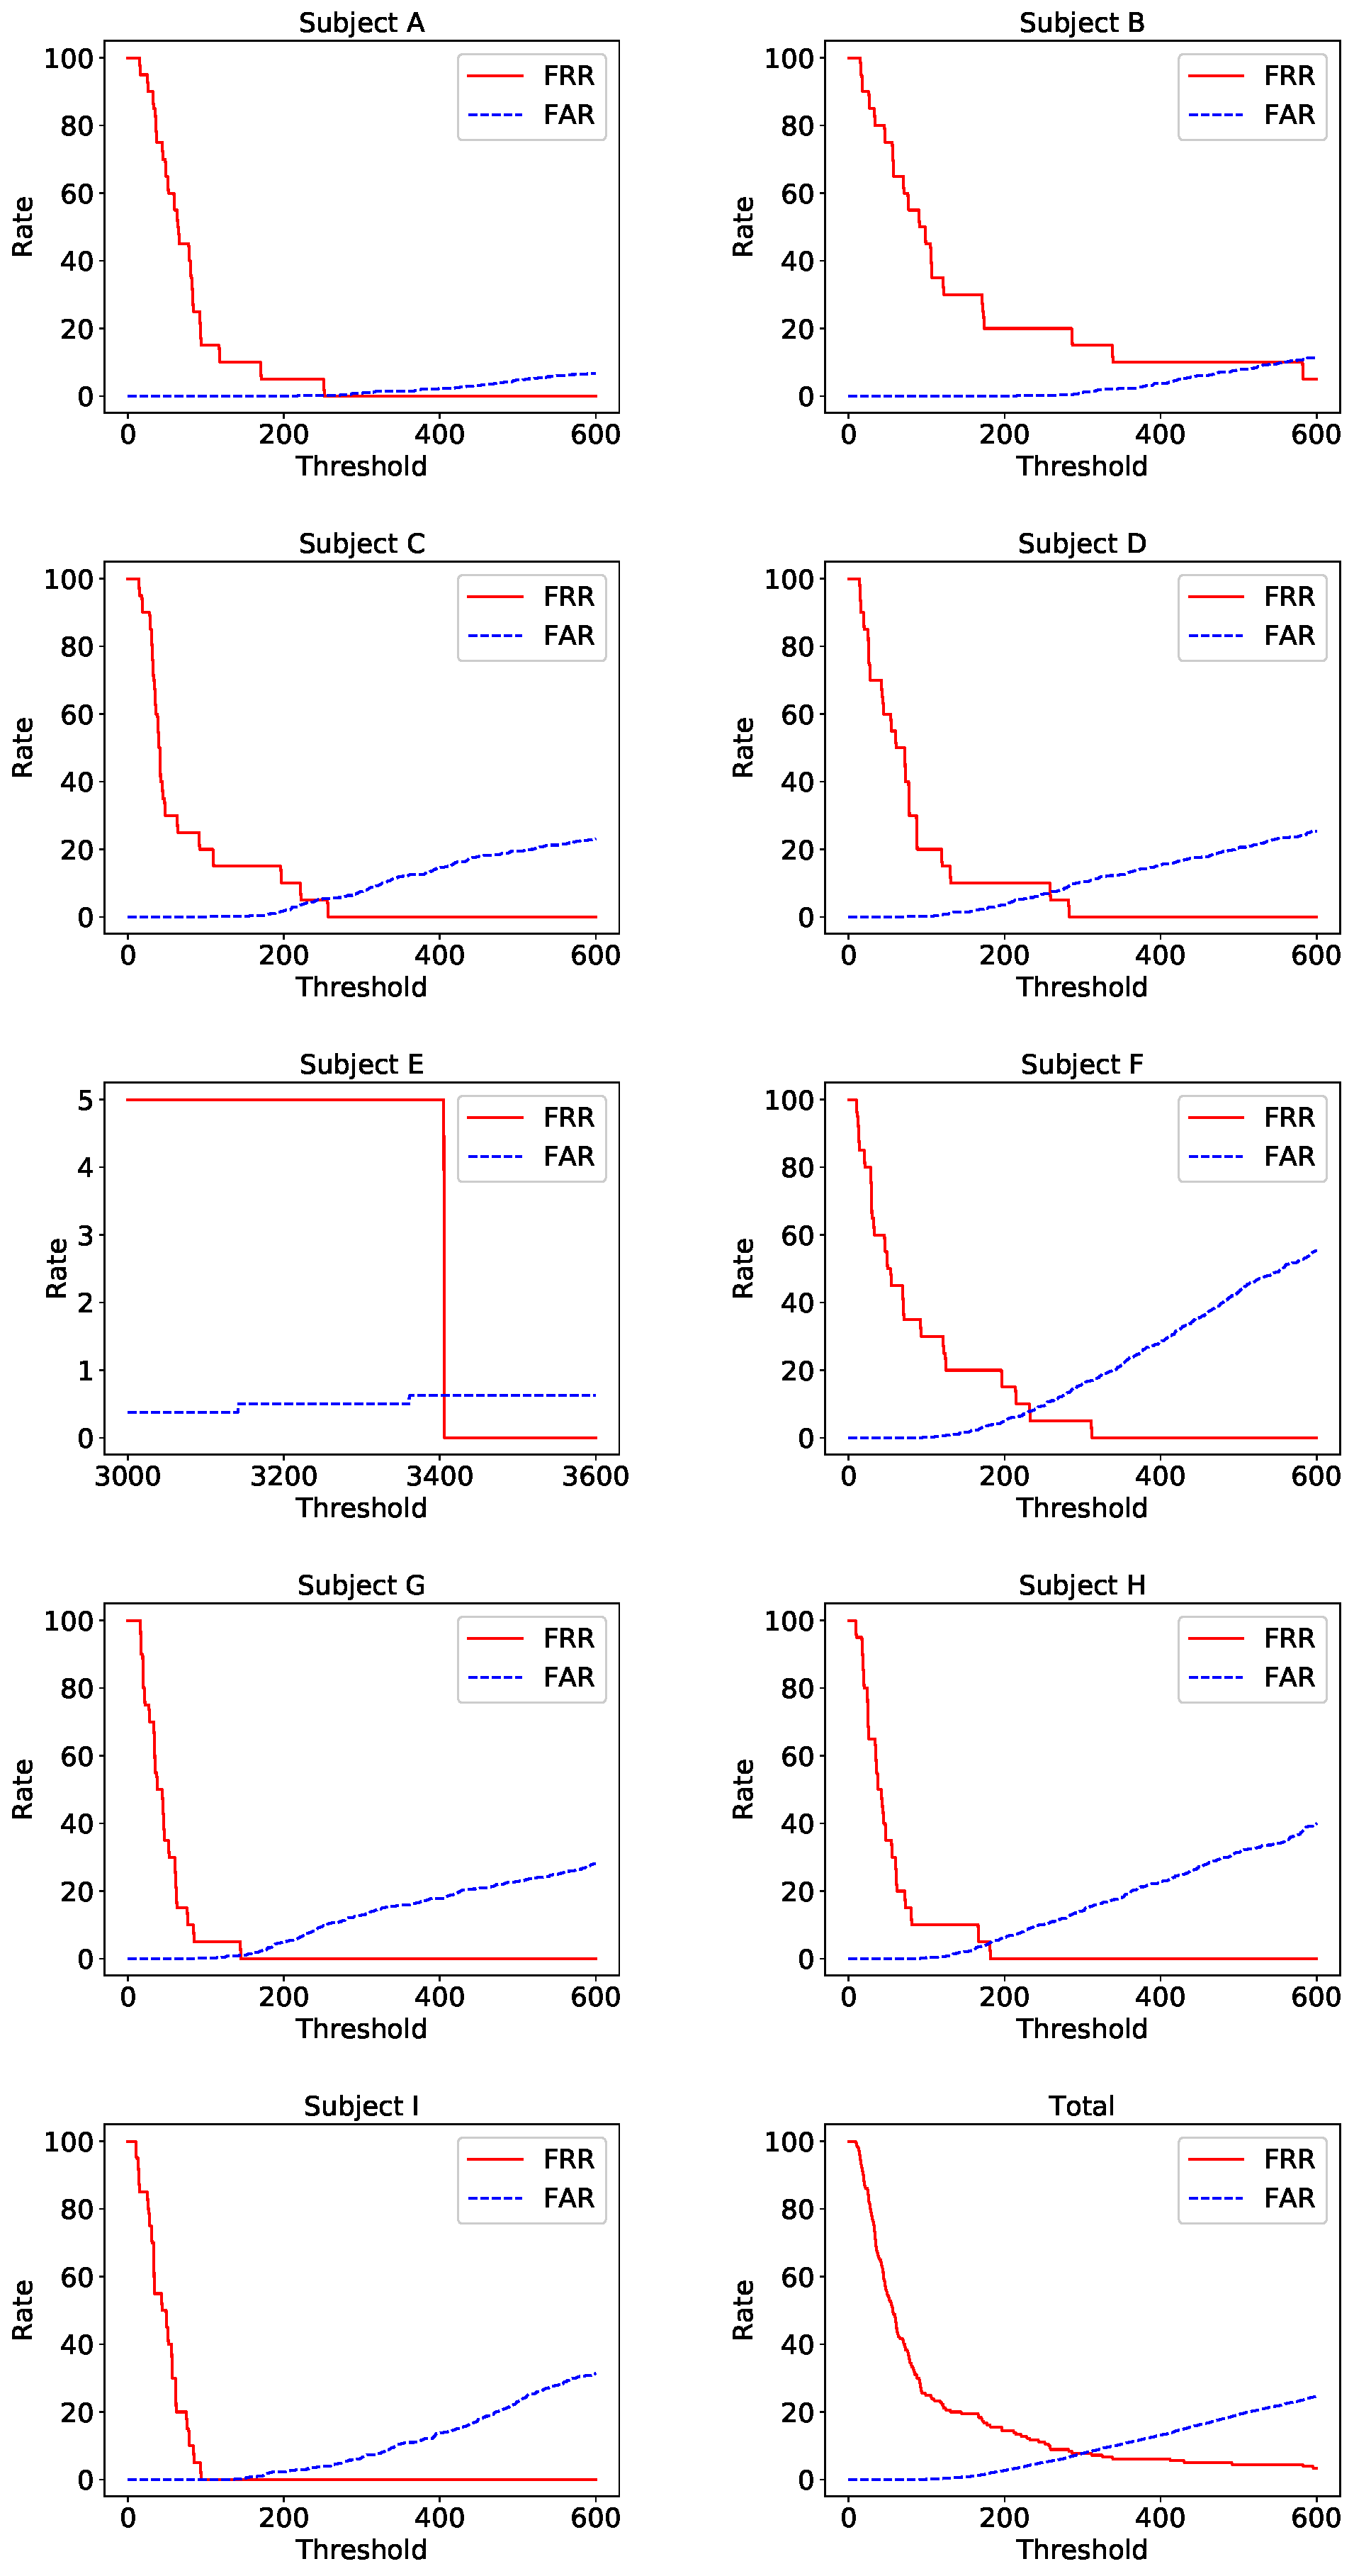
\includegraphics[width=0.70\linewidth]{figure/EER.eps}
  \caption{被験者ごとの判別結果}
  \label{EER}
\end{figure}

\begin{figure}[!t]
  \centering
    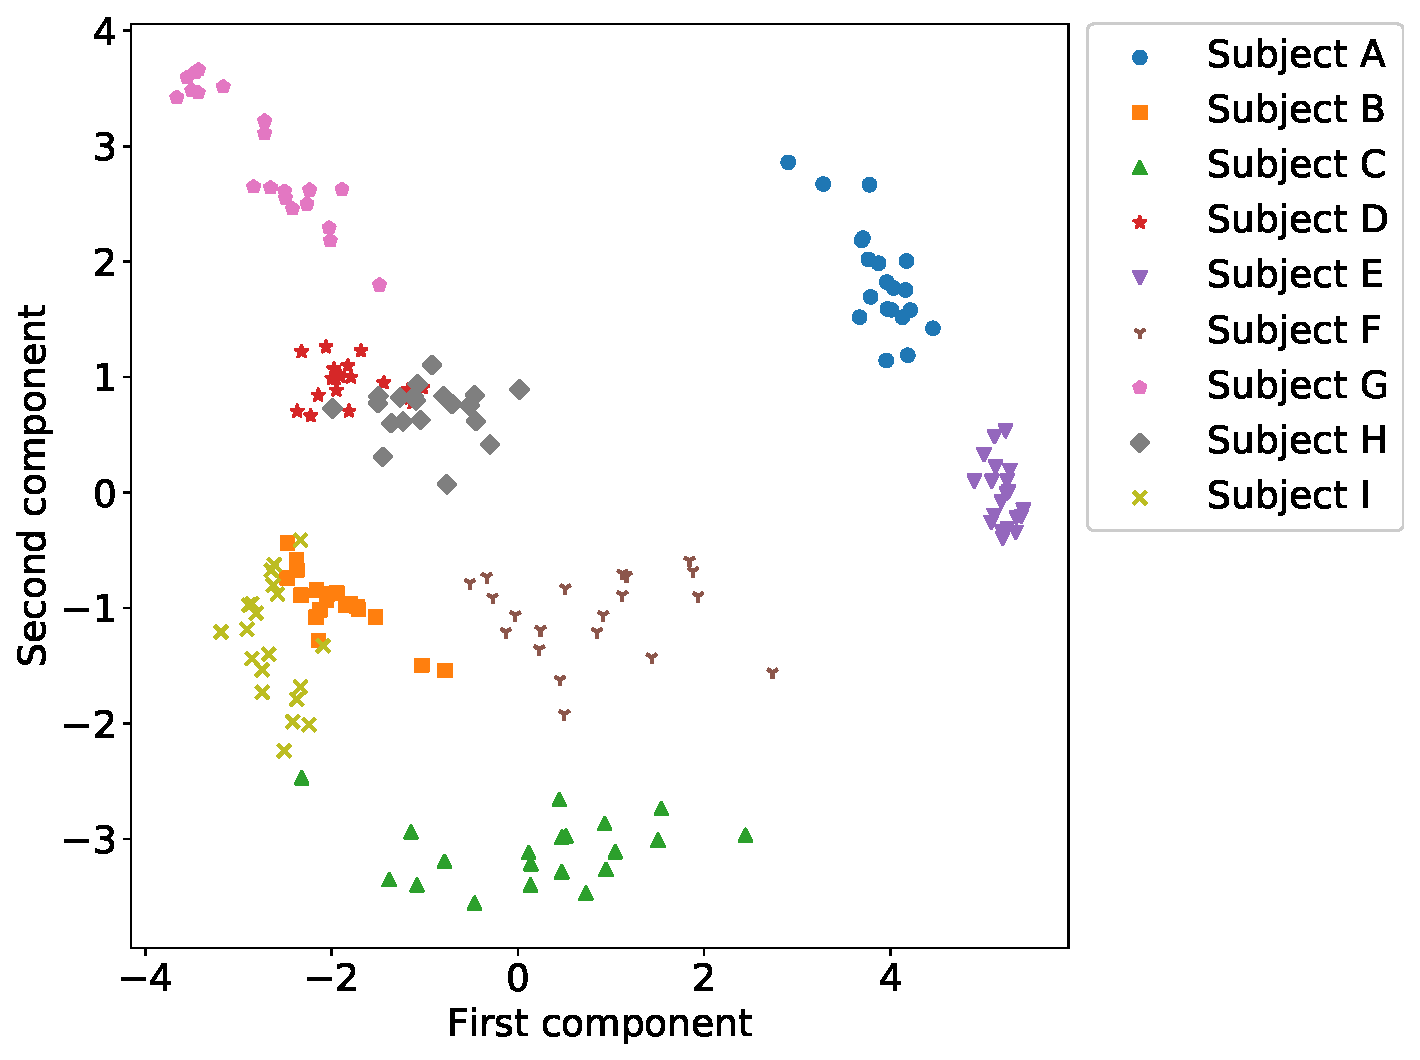
\includegraphics[width=1\linewidth]{figure/PCA.eps}
  \caption{PCAによる分析結果}
  \label{PCA}
\end{figure}
\chapter{Limitations}
\label{sec:limitation}
The results in Chapter \ref{sec:evaluation} showed that the measured heart rate could be input to the smartwatch with small errors in most cases. This chapter discusses the limitations of the proposed method in terms of other pulse-wave-related indices and the pulse waveform.\par

For comparison, I acquired real raw PPG data from my left index finger and raw PPG data generated by display D with a 2-mm acrylic plate. Figure \ref{fig:raw_data_acquisition} illustrates the environment during this raw pulse data acquisition. Numerical pulse data was collected at a sampling rate of 106 Hz for 60 s by using an Arduino Uno R3 and a PPG sensor\footnote{\url{https://www.pulsesensor.com}}. The Arduino used here was different from the one used to control the display.

\begin{figure}[!t]
  \centering
  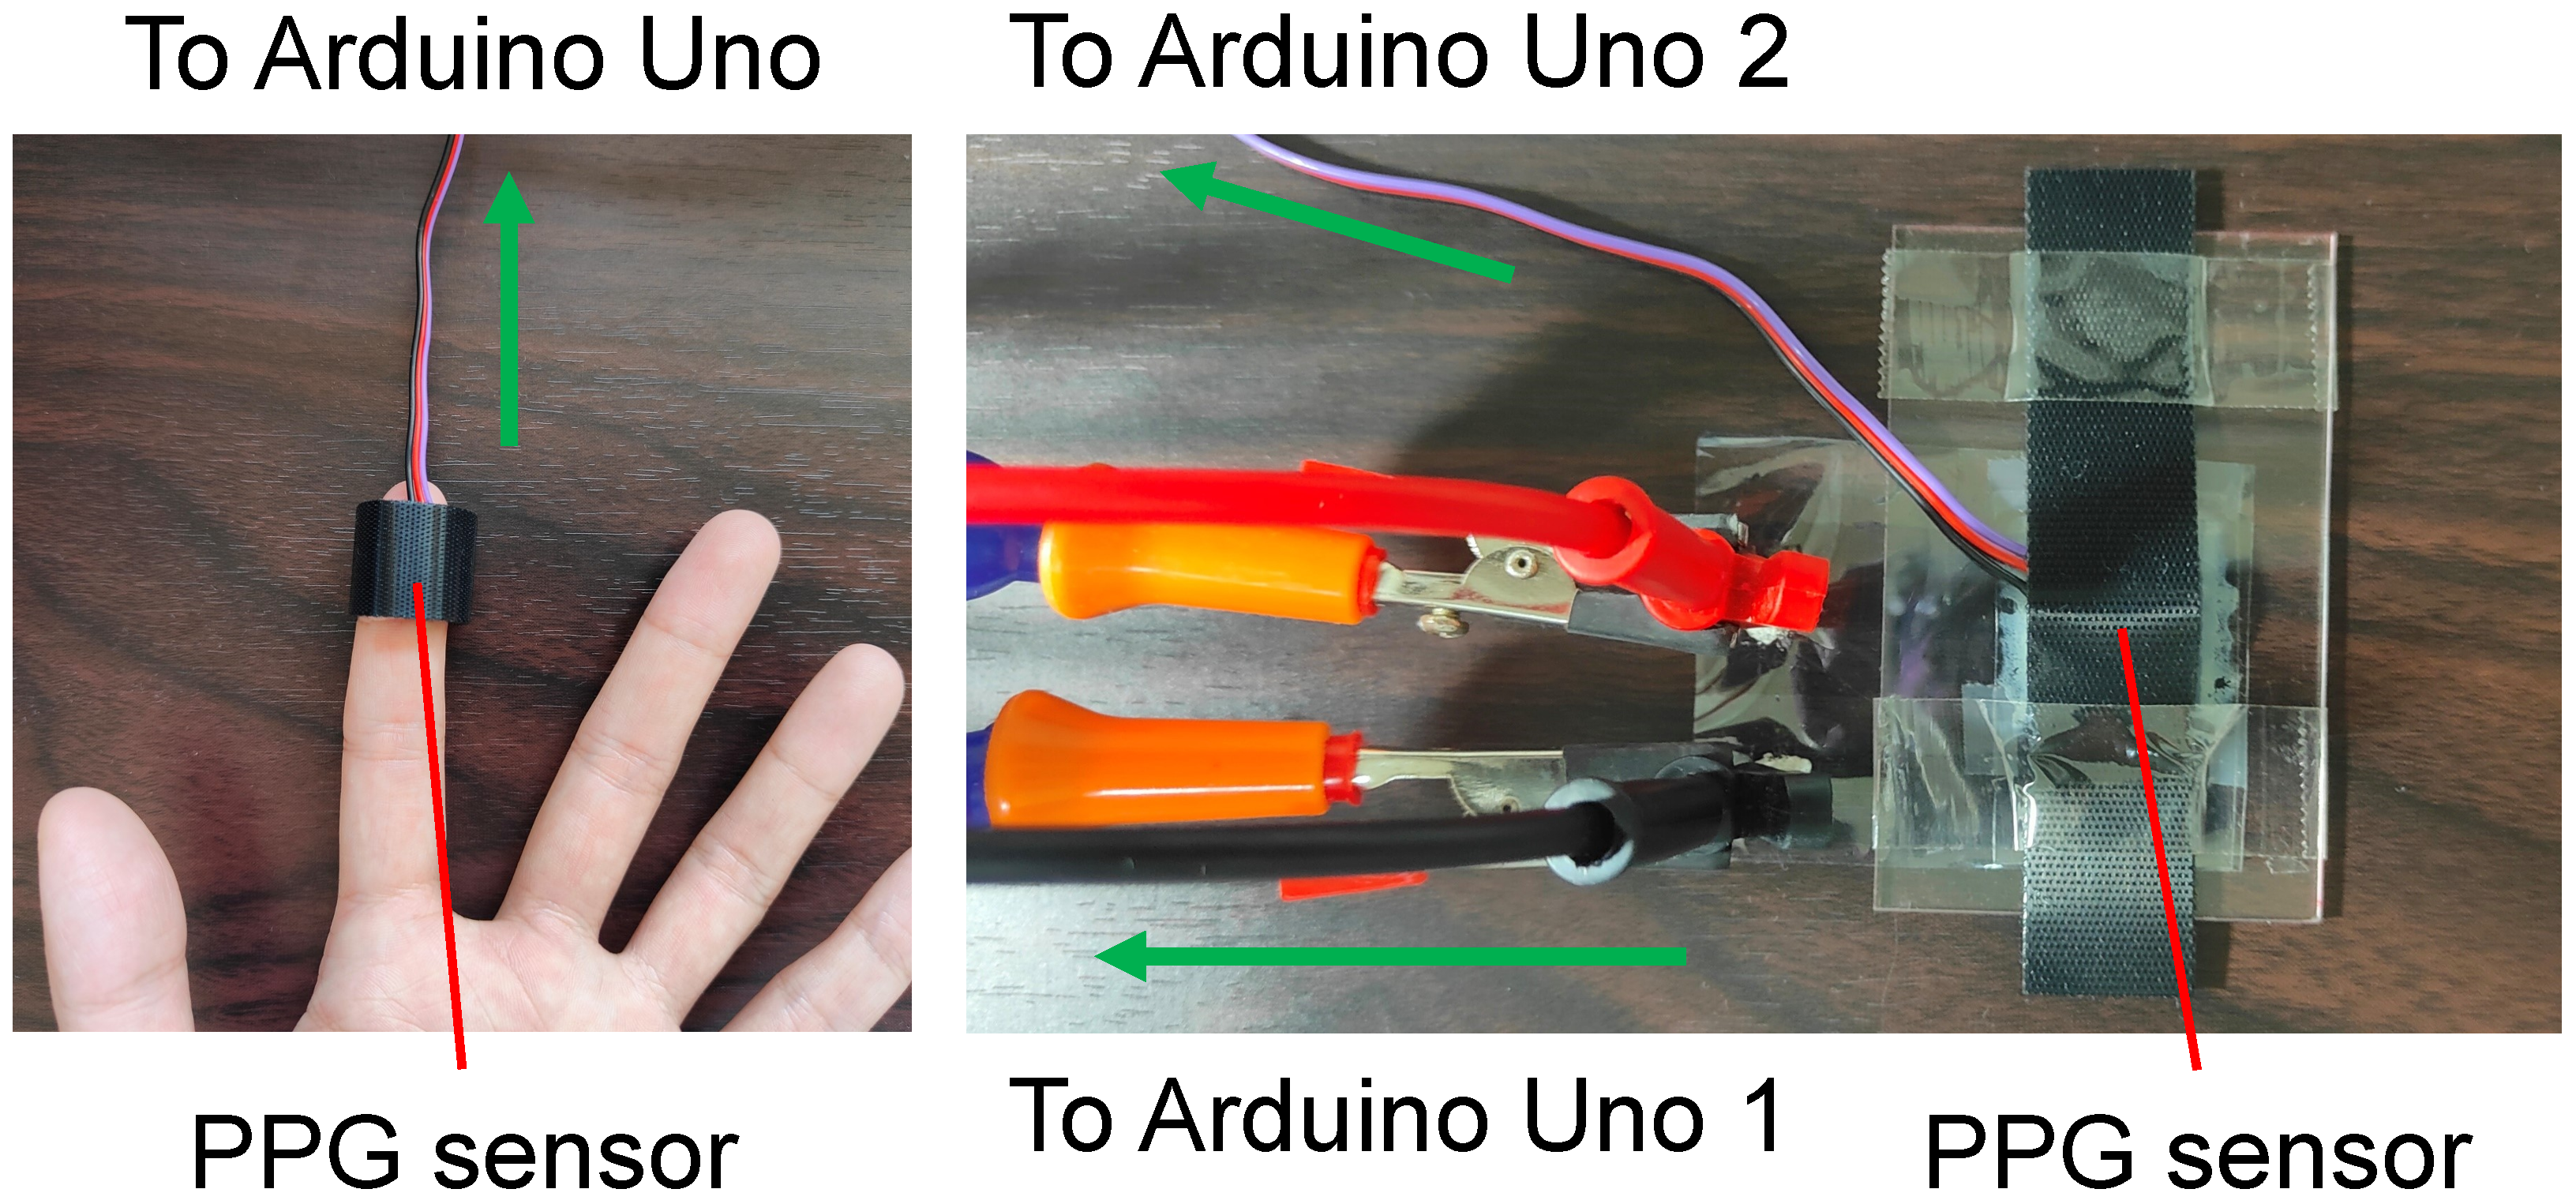
\includegraphics[width=1\linewidth]{figures/raw_data_acquisition.eps}
  \caption{Environment during raw pulse data acquisition.}
  \label{fig:raw_data_acquisition}
\end{figure}


% 5.1
\section{Pulse Wave Status Indicators}
The raw PPG data was analyzed using Kubios HRV Premium (ver. 3.5.0)\footnote{\url{https://www.kubios.com/hrv-premium}}, a fully featured heart rate variability (HRV) analysis software package. Figure \ref{fig:rr_wave} shows the resulting RR time series data, Table \ref{tab:report_real} lists the analysis results for the real PPG data, and Table \ref{tab:report_generated} lists the results for the generated PPG data. The values in these analysis results were calculated from the RR time series data. The target heart rate at the time of pulse wave generation was set to 68 bpm, which was the mean heart rate (HR) of the real pulse wave obtained from the finger.\par

The results showed that the generated pulse wave was at 68 bpm for both the minimum HR and the maximum HR. They also showed that the target heart rate could be input to the PPG sensor in a stable manner, as in the main experiment described in Chapter \ref{sec:evaluation}. As for the RR interval, it is regular under normal conditions but generally varies during relaxation, when the heart is less active. In these results, the mean RR was normal and close between the real and generated pulse waves, which indicates that the generated pulse wave could be recognized as a correct pulse waveform. The standard deviation of the RR interval, denoted as SDNN, was very small for the generated pulse wave. The reason might be that, because the mechanically generated pulse wave was a stable waveform, there was no variation in the RR intervals; this was confirmed by the results shown in Figure \ref{fig:rr_wave}.\par

In pulse wave data, the low-frequency power (LF) indicates both sympathetic and parasympathetic nervous system activity, while the high-frequency power (HF), also known as respiratory sinus arrhythmia (RSA), indicates parasympathetic activity and variation of the RR intervals with respiration. The heart rate increases with inhalation and decreases with exhalation. Because LF appears regardless of whether the sympathetic or parasympathetic nervous system is dominant, the ratio of LF to HF (LF/HF ratio) is used as a stress indicator. In a relaxed state, the parasympathetic nervous system is activated, which results in HF indicating respiratory variations and LF indicating blood pressure variations. On the other hand, under stressful conditions, the sympathetic nervous system is activated, and LF still appears but HF decreases. Therefore, HF is relatively larger in a relaxed state, so the LF/HF ratio is small, while LF is relatively larger in a stressed state, so the LF/HF ratio is large. However, the criterion of the LF/HF ratio for judging stressful conditions depends on individual differences and the measurement conditions. The results here for the power (\%) and the LF/HF ratio of the generated pulse wave showed that HF was large, which indicated a relaxed state. However, this result was inconsistent with the small variation in the RR interval. Because the generated PPG data was not intended to control LF and HF, these values merely resulted from the frequency analysis of the RR interval data, and they may be meaningless. If I can generate more detailed PPG data in the future, it may become possible to control the LF/HF ratio.

\begin{figure*}[!t]
  \centering
  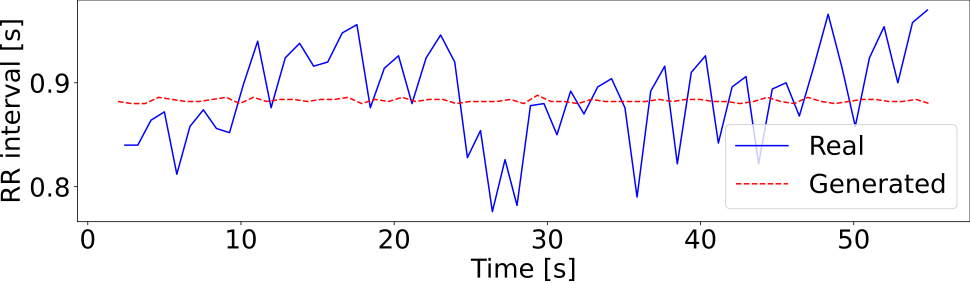
\includegraphics[width=1\linewidth]{figures/rr_wave.eps}
  \caption{RR time series data.}
  \label{fig:rr_wave}
\end{figure*}

\begin{table*}[!t]
  \centering
  \caption{Analysis results for the real PPG data.}
  \begin{minipage}[t]{1\linewidth}
    \centering
    \subcaption{Time-Domain Results}
    \begin{tabular}{lrr}
    \toprule
    Variable & Units & Value \\
    \midrule
    Mean RR & (ms) & $887$ \\
    Mean HR & (bpm) & $68$ \\
    Min HR & (bpm) & $63$ \\
    Max HR & (bpm) & $74$ \\
    SDNN & (ms) & $37.5$ \\
    RMSSD & (ms) & $49.4$ \\
    NN50 & (beats) & $20$ \\
    pNN50 & (\%) & $33.90$ \\
    RR triangular index & & $7.50$ \\
    TINN & (ms) & $149.0$ \\
    Stress Index (SI) & & $12.8$ \\
    DC & (ms) & $26.6$ \\
    DCmod & (ms) & $51.4$ \\
    \bottomrule
    \end{tabular}
    \vspace{10pt}
  \end{minipage}
  \begin{minipage}[t]{1\linewidth}
    \centering
    \subcaption{Frequency-Domain Results (FFT spectrum)}
    \begin{tabular}{lrrrr}
    \toprule
    Variable & Units & VLF & LF & HF \\
    \midrule
    Frequency band & (Hz) & $0.00\text{--}0.04$ & $0.04\text{--}0.15$ & $0.15\text{--}0.40$ \\
    Peak frequency & (Hz) & $0.040$ & $0.113$ & $0.350$ \\
    Power & (ms${}^\text{2}$) & $113$ & $800$ & $657$ \\
    Power & (log) & $4.726$ & $6.684$ & $6.488$ \\
    Power & (\%) & $7.17$ & $50.84$ & $41.79$ \\
    Power & (n.u.) & & $54.77$ & $45.02$ \\
    \text{-}\text{-}\text{-}\text{-}\text{-}\text{-}\text{-}\text{-}\text{-}\text{-}\text{-}\text{-}\text{-} & & & & \\
    Total power & (ms${}^\text{2}$) & $1573$ & & \\
    Total power & (log) & $7.361$ & & \\
    LF/HF ratio & & $1.216$ & & \\
    RESP & (Hz) & $-$ & & \\
    \bottomrule
    \end{tabular}
  \end{minipage}
  \label{tab:report_real}
\end{table*}

\begin{table*}[!t]
  \centering
  \caption{Analysis results for the generated PPG data.}
  \begin{minipage}[t]{1\linewidth}
    \centering
    \subcaption{Time-Domain Results}
    \begin{tabular}{lrr}
    \toprule
    Variable & Units & Value \\
    \midrule
    Mean RR & (ms) & $883$ \\
    Mean HR & (bpm) & $68$ \\
    Min HR & (bpm) & $68$ \\
    Max HR & (bpm) & $68$ \\
    SDNN & (ms) & $1.9$ \\
    RMSSD & (ms) & $3.1$ \\
    NN50 & (beats) & $0$ \\
    pNN50 & (\%) & $0.00$ \\
    RR triangular index & & $NaN$ \\
    TINN & (ms) & $7.0$ \\
    Stress Index (SI) & & $81.7$ \\
    DC & (ms) & $1.0$ \\
    DCmod & (ms) & $3.2$ \\
    \bottomrule
    \end{tabular}
    \vspace{10pt}
  \end{minipage}
  \begin{minipage}[t]{1\linewidth}
    \centering
    \subcaption{Frequency-Domain Results (FFT spectrum)}
    \begin{tabular}{lrrrr}
    \toprule
    Variable & Units & VLF & LF & HF \\
    \midrule
    Frequency band & (Hz) & $0.00\text{--}0.04$ & $0.04\text{--}0.15$ & $0.15\text{--}0.40$ \\
    Peak frequency & (Hz) & $0.030$ & $0.120$ & $0.287$ \\
    Power & (ms${}^\text{2}$) & $0$ & $0$ & $1$ \\
    Power & (log) & $0.000$ & $0.000$ & $0.088$ \\
    Power & (\%) & $1.64$ & $25.16$ & $73.00$ \\
    Power & (n.u.) & & $25.57$ & $74.22$ \\
    \text{-}\text{-}\text{-}\text{-}\text{-}\text{-}\text{-}\text{-}\text{-}\text{-}\text{-}\text{-}\text{-} & & & & \\
    Total power & (ms${}^\text{2}$) & $1$ & & \\
    Total power & (log) & $0.403$ & & \\
    LF/HF ratio & & $0.345$ & & \\
    RESP & (Hz) & $-$ & & \\
    \bottomrule
    \end{tabular}
  \end{minipage}
  \label{tab:report_generated}
\end{table*}


% 5.2
\section{Pulse Waveform}
The first 10 s of the real and generated raw PPG data are plotted in Figure \ref{fig:raw_wave}. The real pulse wave varied in amplitude and was not stable. In contrast, the generated pulse wave had a stable waveform but its similarity to the real pulse waveform was low. Even an irregular waveform can be recognized as a pulse wave by the smartwatch and analysis software, and indicators such as the heart rate can be calculated. Accordingly, because the calculation of the pulse wave status indicators depends on the algorithm of each product in the system, it is necessary to check the raw data waveform to verify that it is genuine PPG data in order to defend against an attack with fake PPG data. As the PPG sensor uses a photoreflector to read changes in light, it is susceptible to the effects of external light due to changes in the mounting position. The optimal $Colors$ array was determined heuristically here, but it is difficult to deal with noise. To address this problem and ensure that generated pulse waveforms resemble real pulse waveforms, it will be necessary to automate the $Colors$ determination process.

\begin{figure*}[!t]
  \centering
  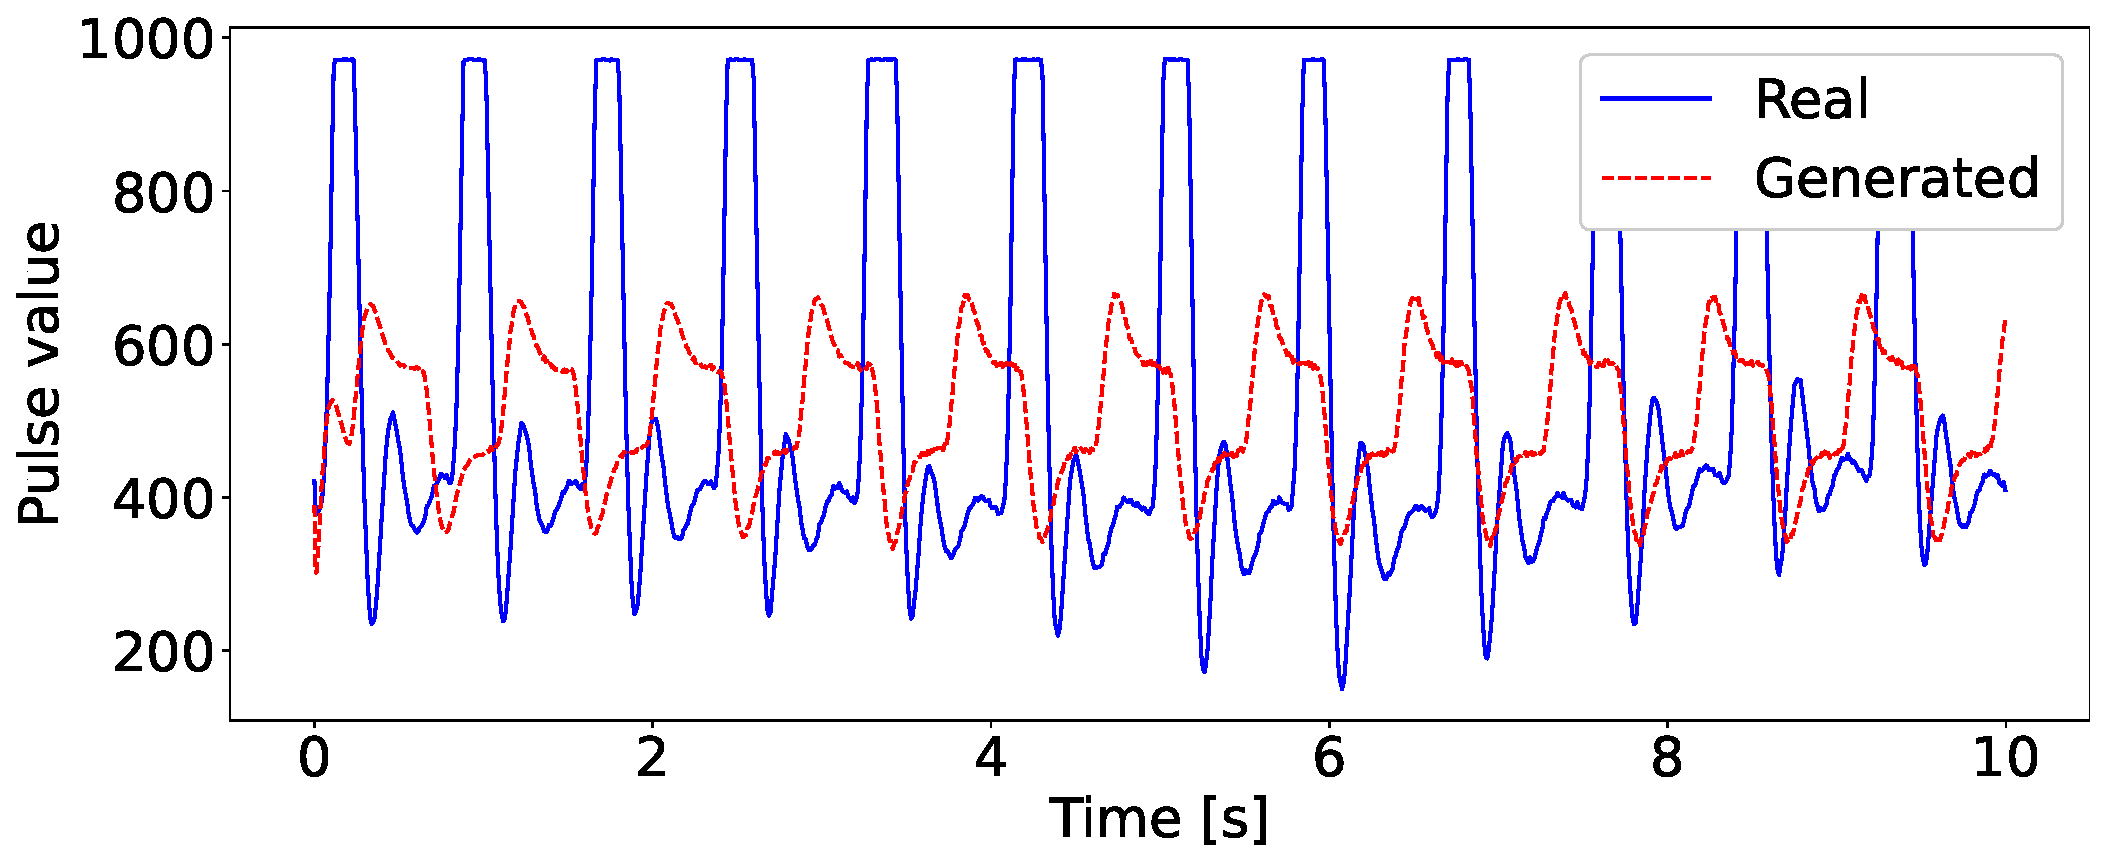
\includegraphics[width=1\linewidth]{figures/raw_wave.eps}
  \caption{Raw PPG data.}
  \label{fig:raw_wave}
\end{figure*}

\chapter{Conclusion}
\label{sec:conclusion}
In this thesis, I proposed a method that enables a PPG sensor to measure an arbitrary pulse wave by using a display. To investigate the effectiveness of the proposed method, I implemented display drawing programs and conducted evaluation experiments with five kinds of smartwatches and four kinds of displays. The results showed that the error between the target heart rate and the heart rate acquired by the smartwatch was within $3$ bpm in many cases when the target heart rate was set to 60--100 bpm. In contrast, when the target heart rate was set to 40--55 and 105--200 bpm, the measured heart rate could be input to the smartwatch with a small error under certain conditions. When the generated PPG data was imported into HRV analysis software, it was recognized as a pulse wave in the same way as real PPG data obtained from a person. By comparing the heart rate, RR interval, and SDNN calculated from the real and generated PPG data, I also confirmed that the proposed method could generate stable PPG data. On the other hand, when the waveforms were compared, the generated PPG waveform differed greatly from the real PPG waveform, which indicated that the software could calculate the heart rate, RR interval, SDNN, and LF/HF ratio regardless of the waveform. This result indicates that calculation of these parameters without verifying the waveform would be vulnerable to an attack with fake PPG data.\par

In my future work, I will improve the reproducibility of PPG data for use in a real environment and implement a mechanism that enables a wearable device on a display to measure the same PPG data by inputting PPG data obtained from a living body part. To achieve this, the system will need to automatically determine the colors to be drawn on the display while calibrating for the environment; I will thus build a generative model that can output the colors to be drawn from input PPG data.


\chapter*{Acknowledgments}
I would like to express my special appreciation and thanks to my advisor Associate Professor Dr. Kazuya Murao, you have been a tremendous mentor for me. I would like to thank you for encouraging my research and for allowing me to grow. Your advice for my research have been invaluable. I would also wish to express my gratitude to Professor Dr. Nobuhiko Nishio and Assistant Professor Dr. Kyosuke Futami for extended discussions and valuable suggestions which have contributed greatly to the improvement of the thesis. I would like to thank Senior Assistant Professor Dr. Naoji Matsuhisa of Electronics and Electrical Engineering, Keio University for providing me with a device implemented with an innovative method and for contributing to my experiments with new ideas. I am also so thankful to my fellow students whose challenges and productive critics, especially at the Murao Laboratoty, have provided new ideas to the work. I also thank my family. This accomplishment would not have been possible without them. Finally, I would like to thank my friends who supported each other in difficult times. Thank you.
\addcontentsline{toc}{chapter}{Acknowledgments}

\bibliographystyle{junsrt}
\bibliography{references}

\end{document}
